
\documentclass[11pt,a4paper]{article}
\usepackage{amsmath,amssymb,physics}
\usepackage{tikz}
\usetikzlibrary{arrows.meta,positioning,patterns,decorations.pathmorphing,calc}
\usepackage{tcolorbox}
\usepackage{tabularx}
\usepackage{microtype}
\usepackage{caption}
\captionsetup{justification=raggedright,singlelinecheck=false}
\usepackage{hyperref}

\title{From Keldysh to L\'evy: Unified EM Noise Framework for Trapped Ions}
\author{Ulrich Warring et al.}
\date{\today}

\begin{document}
\maketitle

\begin{abstract}
We derive a unified first-principles description of motional heating in trapped ions by integrating out electromagnetic degrees of freedom in the Keldysh formalism. 
All noise mechanisms---technical field fluctuations and collisional impulses---enter through stochastic current sources coupled via the trap's Green tensor. 
The resulting open-system dynamics take the form of a L\'evy--Khintchine generator (Gaussian diffusion + compound-Poisson jumps), with explicit links to scattering cross-sections. 
We provide experimentally discriminating observables, scattering-model formulas, and a practical inference protocol for reconstructing the jump-size L\'evy measure from stroboscopic measurements.
\end{abstract}

\tableofcontents

\input{introduction}
\input{theory_sections}
\input{discriminants_table}
\section{Observable Signatures and Scattering Models}
The unified L\'evy--Khintchine generator (Eq.~\ref{eq:levy-box}, Sec.~2.6) predicts 
that ion heating arises from a combination of Gaussian diffusion and compound-Poisson jumps. 
We now develop experimentally distinguishable signatures that allow independent extraction of these components.

\noindent\textbf{(a) Langevin induced-dipole scattering}\quad
\emph{Regime:} Low-energy ion--neutral collisions with polarizable neutral ($E \lesssim 1$~eV).\\
\emph{Cross-section:}
\[
\frac{d\sigma}{d\Omega} = 
\frac{\alpha e^2}{8\pi\epsilon_0^2 \mu^2 v^4}\,
\frac{\sin^2\theta}{(1-\cos\theta)^4},
\]
with $\alpha$ the neutral polarizability. The total Langevin cross-section is 
$\sigma_{\rm L} = \pi e\sqrt{\alpha/(\epsilon_0 E)} \propto E^{-1/2}$.\\
\emph{Key feature:} Soft divergence at small $\Delta p$ (forward scattering), cut off by quantum diffraction $b_{\min}\sim \hbar/\mu v$.\\
\emph{Consequence:} $\nu(\Delta p)$ has enhanced small-$\Delta p$ weight; CLT $\to$ near-Gaussian heating but with fat tails.\\
\emph{Relevant systems:} Ca$^+$/Sr$^+$/Ba$^+$ with H$_2$, N$_2$, Ar backgrounds.

\textit{Universal behavior:} 
The Langevin form is \emph{universal} in the sense that it depends only on the neutral's polarizability $\alpha$, not on molecular details. 
This implies that $\nu(\Delta p)$ is parametrized by just $\alpha$ and the velocity distribution $f(v)$, reducing the inference problem to fitting $\lambda$ (or equivalently $n_g$) and $T$ from experimental data.
Departures from universality—resonant charge exchange, short-range chemistry, or high-energy collisions—introduce additional structure in $\nu(\Delta p)$ and require species-specific cross-sections.

\medskip
\noindent\textbf{(b) Hard-sphere scattering}\quad
\emph{Regime:} Classical collisions with effective radius $R$.\\
\emph{Cross-section:}
\[
\frac{d\sigma}{d\Omega} = \frac{R^2}{4\pi}.
\]
\emph{Key feature:} Isotropic scattering, momentum transfer peaked at $|\Delta p|=2\mu v$.\\
\emph{Consequence:} $\nu(\Delta p)$ becomes sharply peaked, yielding bimodal $P(\Delta n)$.\\
\emph{Relevant systems:} Test gases (He, Ne) in controlled background studies.

\medskip
\noindent\textbf{(c) Resonant charge-exchange}\quad
\emph{Regime:} Ion--atom collisions with same species (e.g.\ Ca$^+$ + Ca).\\
\emph{Cross-section:}
\[
\sigma(v) \approx \frac{\pi a_0^2}{1+(v/v_0)^2},
\]
with $v_0\sim \sqrt{\Delta E/\mu}$ from state energy defect $\Delta E$.\\
\emph{Key feature:} Strong velocity dependence; event rate $\lambda\propto n_g\langle v\sigma(v)\rangle$ inherits thermal modulation.\\
\emph{Consequence:} Waiting-time distribution becomes $T$-dependent; seasonal/diurnal modulations possible.\\
\emph{Relevant systems:} Ca$^+$, Yb$^+$ with neutral Ca, Yb vapor.

\medskip
\noindent\textbf{(d) Coulomb scattering (stray charges)}\quad
\emph{Regime:} Fly-by electrons/ions at distance $b\gg L_{\rm trap}$.\\
\emph{Cross-section:} Rutherford form,
\[
\frac{d\sigma}{d\Omega} \propto \frac{1}{\sin^4(\theta/2)}.
\]
\emph{Key feature:} Extremely long range; strong small-angle divergence.\\
\emph{Consequence:} Dominates if stray charges or cosmic rays penetrate; leads to anisotropic heating.\\
\emph{Relevant systems:} Cosmic ray backgrounds, photoionization byproducts.

\section{Spatial Coherence Effects}

\begin{tcolorbox}[title=Fast scatterers: spatial coherence effects]
For a moving scatterer with trajectory 
$\mathbf{r}_k(t)=\mathbf{r}_0+\mathbf{v}t$, 
the current density is
\[
\mathbf{j}_k(\mathbf{r},t) = \mathbf{j}^{(0)}_k(t)\,
\delta^{(3)}(\mathbf{r}-\mathbf{r}_k(t)).
\]
The force spectrum becomes
\[
F_k(\omega) = q \int dt\, e^{i\omega t}\,
\mathbf{G}(\mathbf{r}_0,\mathbf{r}_k(t);\omega)\cdot
\mathbf{j}^{(0)}_k(t).
\]

\textbf{Velocity regimes:}
\begin{itemize}\itemsep0.2em
\item Thermal background ($v \sim 500$~m/s, $\tau_{\rm coll}\sim 10$~ps): 
$v\tau_{\rm coll}\sim 5$~nm $\ll L_{\rm trap}$ $\to$ point-impulse limit.
\item Fast cosmics ($v\sim 0.1c$, $\tau_{\rm coll}\sim 1$~ps): 
$v\tau_{\rm coll}\sim 30~\mu$m $\sim L_{\rm trap}$ $\to$ extended-coherence regime.
\end{itemize}

\textbf{Impact:} Spatial variation of $\mathbf{G}$ introduces directional coupling, 
$|F_k(\omega)|^2 \propto |\hat{\mathbf{v}}\cdot\nabla\mathbf{G}|^2$, 
breaking isotropy. 

\textbf{Observable:} Anisotropic heating as a function of trap orientation relative to a collimated beam or fast flux (see Fig.~\ref{fig:trajectory_coherence}).
\end{tcolorbox}
\begin{figure}[h]
\centering
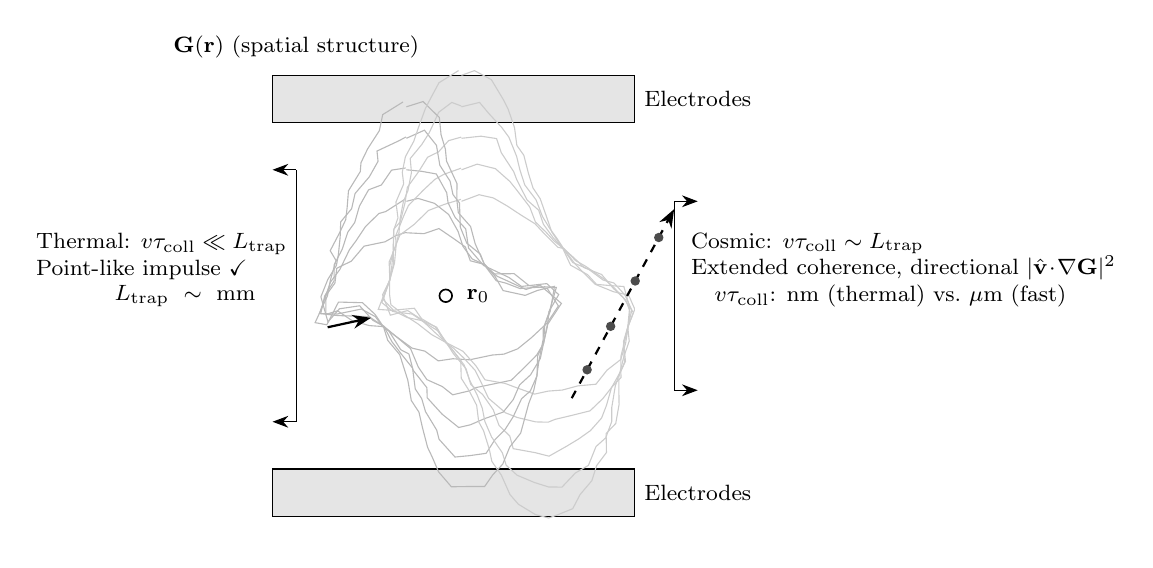
\begin{tikzpicture}[x=1cm,y=1cm,>=Stealth]
  \small
  \def\W{4.6}
  \def\H{6.2}
  \def\gap{3.2}
  \node at (0,0) {};
  \draw[fill=gray!20] (-1.5,  \gap/2+0.6) rectangle (\W-1.5,  \gap/2+1.2);
  \draw[fill=gray!20] (-1.5, -\gap/2-1.2) rectangle (\W-1.5, -\gap/2-0.6);
  \node[font=\footnotesize] at (\W-1.5+0.8,  \gap/2+0.9) {Electrodes};
  \node[font=\footnotesize] at (\W-1.5+0.8, -\gap/2-0.9) {Electrodes};
  \begin{scope}
    \clip (-1.5, -\H/2) rectangle (\W-1.5, \H/2);
    \foreach \a in {0.8,1.2,1.6,2.0,2.4}{
      \draw[gray!55, decorate, decoration={random steps, segment length=2mm, amplitude=0.6mm}]
        plot[smooth cycle, tension=1] coordinates{
          (-0.8,0) (0.2,\a) (1.2,0.4) (2.0,-0.2) (1.0,-\a) (-0.1,-0.4)};
      \draw[gray!40, decorate, decoration={random steps, segment length=2mm, amplitude=0.5mm}]
        plot[smooth cycle, tension=1] coordinates{
          (0.0,0.2) (0.9,\a+0.4) (2.2,0.6) (3.0,-0.4) (2.0,-\a-0.4) (0.7,-0.6)};
    }
  \end{scope}
  \node[font=\footnotesize, anchor=south] at (-1.2, \H/2-0.2) {$\mathbf{G}(\mathbf{r})$ (spatial structure)};
  \filldraw[fill=white, draw=black, line width=0.6pt] (0.7,0) circle (0.08);
  \node[font=\footnotesize, anchor=west] at (0.85,0) {$\mathbf{r}_0$};
  \draw[thick, -Stealth] (-0.8, -0.4) -- ++(0.55,0.12);
  \node[font=\footnotesize, align=left, anchor=east] at (-1.2,0.5)
    {Thermal: $v\tau_{\rm coll} \ll L_{\rm trap}$\\Point-like impulse \checkmark};
  \draw[thick, dashed, -Stealth] (2.3, -1.3) -- (3.6, 1.1);
  \foreach \t in {0.15,0.38,0.62,0.85}{
    \fill[black!70] ($(2.3, -1.3)!{\t}!(3.6,1.1)$) circle (0.06);
  }
  \node[font=\footnotesize, align=left, anchor=west] at (3.7, 0.5)
    {Cosmic: $v\tau_{\rm coll} \sim L_{\rm trap}$\\Extended coherence, directional $|\hat{\mathbf{v}}\!\cdot\!\nabla\mathbf{G}|^2$};
  \draw[very thin] (-1.2,-\gap/2) -- (-1.2,\gap/2);
  \draw[-{Stealth[length=2mm]}] (-1.2,\gap/2) -- ++(-0.3,0);
  \draw[-{Stealth[length=2mm]}] (-1.2,-\gap/2) -- ++(-0.3,0);
  \node[font=\footnotesize, align=center, anchor=east] at (-1.6,0) {$L_{\rm trap}\ \sim\ \mathrm{mm}$};
  \draw[very thin] (\W-1.0,-1.2) -- (\W-1.0,1.2);
  \draw[-{Stealth[length=2mm]}] (\W-1.0,1.2) -- ++(0.3,0);
  \draw[-{Stealth[length=2mm]}] (\W-1.0,-1.2) -- ++(0.3,0);
  \node[font=\footnotesize, align=center, anchor=west] at (\W-0.6,0)
    {$v\tau_{\rm coll}$: nm (thermal) vs.\ $\mu$m (fast)};
\end{tikzpicture}

\caption{%
\textbf{Spatial coherence effects for fast scatterers.}
When the trajectory extent $v\tau_{\rm coll}$ approaches the trap dimension $L_{\rm trap}$, $\mathbf{G}(\mathbf{r})$ varies along the path, leading to directional coupling $|F_k(\omega)|^2 \propto |\hat{\mathbf{v}}\!\cdot\!\nabla\mathbf{G}|^2$ and anisotropic heating.}
\label{fig:trajectory_coherence}
\end{figure}
\section{Inference Protocol}

\paragraph{Recommended stroboscopic sequence.}
\begin{enumerate}\itemsep0.2em
  \item Prepare motional ground state $\lvert n=0\rangle$ (or a calibrated thermal $\langle n\rangle$).
  \item Wait time $\tau$ (free evolution under noise).
  \item Read out $n$ via sideband thermometry or time-of-flight.
  \item Repeat $N$ times $\Rightarrow$ histogram $P(n\,|\,\tau)$ and time series $n(t)$.
\end{enumerate}

\paragraph{Sample-size guidelines.}
\begin{table}[h]
\centering
\renewcommand{\arraystretch}{1.15}
\begin{tabularx}{0.9\textwidth}{>{\raggedright\arraybackslash}X>{\raggedleft\arraybackslash}p{4.2cm}}
\hline
\textbf{Target quantity} & \textbf{Required shots/events (order-of-magnitude)} \\
\hline
Detect $\kappa_3 \neq 0$ at $3\sigma$ & $\sim 10^4$ stroboscopic shots \\
Reconstruct $\nu(\Delta n)$ (5 bins)  & $\sim 10^5$ shots \\
Test heavy-tail exponent $\alpha$      & $\sim 10^6$ events \\
Allan variance rollover near $1/\lambda$ & hours of continuous trace \\
Sideband asymmetry vs.\ $\omega$ map   & $\sim 10^2$ frequency scans \\
\hline
\end{tabularx}
\end{table}

\paragraph{Systematic error sources (and mitigations).}
\begin{itemize}\itemsep0.2em
  \item \textbf{Readout noise} smears $P(\Delta n)$: calibrate with known coherent kicks and deconvolve.
  \item \textbf{Motional dephasing} during $\tau$: ensure $\tau \ll 1/\Gamma_{\rm dephase}$ or include dephasing in the likelihood model.
  \item \textbf{Multi-ion coupling}: analyze in normal-mode basis; report mode-resolved $\nu(\Delta n)$.
  \item \textbf{Background drift / non-stationarity}: use sliding-window estimators for $\lambda(t)$, $\langle \Delta n \rangle(t)$.
\end{itemize}

\paragraph{Estimation outputs (minimum set).}
\begin{itemize}\itemsep0.2em
  \item Cumulants $\kappa_2(\tau)$, $\kappa_3(\tau)$, $\kappa_4(\tau)$; Gaussian vs.\ non-Gaussian decision.
  \item Change-point inference of jump times $\{t_k\}$ and sizes $\{\Delta n_k\}$; empirical $\hat{\nu}(\Delta n)$.
  \item Rollover in $\sigma_A^2(\tau)$ and sideband asymmetry vs.\ $\omega$ to constrain $|\mathbf{G}(\omega)|^2$.
\end{itemize}% Inference protocol placeholder

\bibliographystyle{unsrt}
\bibliography{refs}
\end{document}
